% Section 2.2: The tensor product | Part: 1 | Depends on: sec:vectors | Status: done | Original lines: 546-653
%!TEX root = ../../main.tex
\subsection{The tensor product}\label{sec:tensorproduct}
\begin{formal}[{tensor product of multilinear maps}]
% REWRITTEN: notation E_i -> V_i, F_j -> W_j (docs/NOTATION.md)
Given multilinear $f:V_1\times\dots\times V_k\to\R$ and $g:W_1\times\dots\times W_\ell\to\R$, their \emph{tensor product} is the multilinear map $f\otimes g:V_1\times\dots\times V_k\times W_1\times\dots\times W_\ell\to\R$,
\[
(f\otimes g)(v_1,\dots,v_k,u_1,\dots,u_\ell)=f(v_1,\dots,v_k)\cdot g(u_1,\dots,u_\ell).
\]
Properties: bilinear and associative, but \textbf{not commutative} in general ($f\otimes g\ne g\otimes f$). If $\{e^{i}\}$ is the dual basis of $V_1$ and $\{f^{j}\}$ that of $V_2$, then $\{e^{i}\otimes f^{j}\}$ is a basis of the space of bilinear maps $V_1\times V_2\to\R$, which is written $V_1^*\otimes V_2^*$; its dimension is $\dim V_1\cdot\dim V_2$.
\end{formal}

\begin{intuition}[{``run both machines side by side and multiply the outputs''}]
$f\otimes g$ is a machine with the hoppers of $f$ followed by the hoppers of $g$. It feeds the first group to $f$, the second group to $g$, and multiplies the two numbers. It is the most ``free'' way to combine two machines: all other bilinear machines are built by \emph{adding} such products. Not every bilinear machine is a single product (the \emph{pure} tensors are discussed after Theorem~\ref{thm:tensorbasis}).
% REWRITTEN: the non-pure example e^1(x)e^2+e^2(x)e^1 is now stated once, after thm:tensorbasis
\end{intuition}

\begin{example}[{tensor product of two covectors on $\R^2$}]
Take $f=e^{1}+2e^{2}$, $g=3e^{1}-e^{2}$. Then
\[
f\otimes g=3\,e^{1}\!\otimes e^{1}-e^{1}\!\otimes e^{2}+6\,e^{2}\!\otimes e^{1}-2\,e^{2}\!\otimes e^{2},
\]
and $(f\otimes g)(v,w)=(v^1+2v^2)(3w^1-w^2)$. Its component matrix $(f_ig_j)=\begin{pmatrix}3&-1\\6&-2\end{pmatrix}$ has rank 1. Contrast $g\otimes f$: components $(g_if_j)=\begin{pmatrix}3&6\\-1&-2\end{pmatrix}$, the transpose.
\end{example}


\subhead{The abstract definition: a universal property}
The functional definition above is convenient for computing. The following characterisation does not depend on any
construction and is the one used to define the algebras of the next sections.

\begin{definition}[Tensor product]\label{def:tensor}
Let $V,W$ be vector spaces. A \emph{tensor product} of $V$ and $W$ is a vector space
$V\otimes W$ together with a bilinear map $\otimes:V\times W\to V\otimes W$,
$(v,w)\mapsto v\otimes w$, such that the following \emph{universal property} holds:
for every vector space $U$ and every bilinear map $\beta:V\times W\to U$ there exists a
\emph{unique linear} map $\tilde\beta:V\otimes W\to U$ with $\beta=\tilde\beta\circ\otimes$.
\[
% Figure | used in parts/01-algebra/02-tensors/02-tensor-product.tex
%!TEX root = ../main.tex
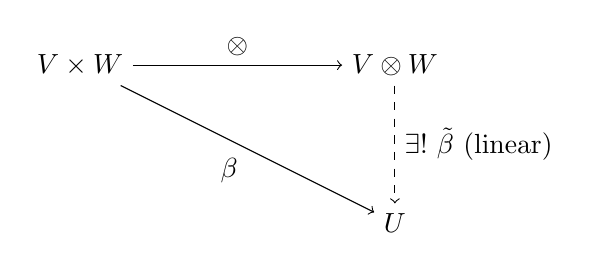
\begin{tikzpicture}[baseline=(current bounding box.center)]
  \node (VW) at (0,0) {$V\times W$};
  \node (T)  at (4,0) {$V\otimes W$};
  \node (U)  at (4,-2) {$U$};
  \draw[->] (VW) -- node[above]{$\otimes$} (T);
  \draw[->] (VW) -- node[below left]{$\beta$} (U);
  \draw[->,dashed] (T) -- node[right]{$\exists!\ \tilde\beta$ (linear)} (U);
\end{tikzpicture}

\]
\end{definition}

In words: \emph{bilinear maps out of $V\times W$ are the same thing as linear maps out of $V\otimes W$}.

\begin{proposition}[Uniqueness]
If $(T_1,\otimes_1)$ and $(T_2,\otimes_2)$ both satisfy Definition~\ref{def:tensor}, there is a unique
linear isomorphism $\phi:T_1\to T_2$ with $\phi(v\otimes_1w)=v\otimes_2w$.
\end{proposition}
\begin{proof}
Apply the universal property of $T_1$ to $\otimes_2$ to get $\phi:T_1\to T_2$, and that of $T_2$ to $\otimes_1$ to get
$\psi:T_2\to T_1$. Then $\psi\circ\phi$ is a linear map $T_1\to T_1$ compatible with $\otimes_1$, as is $\id_{T_1}$;
by the uniqueness clause they coincide. Likewise $\phi\circ\psi=\id_{T_2}$.
\end{proof}

% REWRITTEN: lead-in sentence added
\emph{Existence.} A tensor product always exists; here is the standard construction.
Let $F(V\times W)$ be the \emph{free vector space} on the \emph{set} $V\times W$: formal finite linear combinations
$\sum_a c_a\,[(v_a,w_a)]$ of the symbols $[(v,w)]$, which are declared linearly independent.
Let $N\subset F(V\times W)$ be the subspace spanned by all elements of the form
\begin{align*}
&[(v+v',w)]-[(v,w)]-[(v',w)], & &[(v,w+w')]-[(v,w)]-[(v,w')],\\
&[(\lambda v,w)]-\lambda[(v,w)], & &[(v,\lambda w)]-\lambda[(v,w)].
\end{align*}
Define $V\otimes W:=F(V\times W)/N$ and $v\otimes w:=[(v,w)]+N$. By construction $\otimes$ is bilinear.
Given a bilinear $\beta$, the linear extension of $[(v,w)]\mapsto\beta(v,w)$ to the free space kills $N$,
hence descends to the unique $\tilde\beta$ required. 

\begin{theorem}[Basis and dimension]\label{thm:tensorbasis}
If $(e_i)_{i\le n}$ and $(f_j)_{j\le m}$ are bases of $V$ and $W$, then $(e_i\otimes f_j)$ is a basis of $V\otimes W$.
In particular $\dim(V\otimes W)=nm$.
\end{theorem}
\begin{proof}[Proof sketch]
\emph{Spanning:} by bilinearity, $(v^ie_i)\otimes(w^jf_j)=v^iw^j\,e_i\otimes f_j$, and elements $v\otimes w$ span $V\otimes W$ by construction.
\emph{Independence:} for each pair $(k,l)$ the map $\beta_{kl}(v,w)=e^k(v)f^l(w)$ is bilinear, so it induces a linear
functional $\tilde\beta_{kl}$ on $V\otimes W$ with $\tilde\beta_{kl}(e_i\otimes f_j)=\delta_{ik}\delta_{jl}$. If $\sum c^{ij}e_i\otimes f_j=0$,
applying $\tilde\beta_{kl}$ gives $c^{kl}=0$.
\end{proof}

A general element is therefore $T=T^{ij}\,e_i\otimes f_j$. Elements of the form $v\otimes w$ are called
\emph{pure} (or decomposable); they are the exception rather than the rule: $e_1\otimes e_2+e_2\otimes e_1$ is not pure
(its coefficient matrix has rank $2$; pure tensors are exactly the rank-$1$ matrices). The same holds for
$e^{1}\otimes e^{2}+e^{2}\otimes e^{1}$, the kind of symmetric ``product'' used for metrics.

\begin{proposition}[Standard identifications (finite dimension)]
\begin{enumerate}
  \item $V\otimes\K\cong V$ and $(U\otimes V)\otimes W\cong U\otimes(V\otimes W)$ (associativity).
  \item $V^*\otimes W\cong\Hom(V,W)$ via $(\varphi\otimes w)(v)=\varphi(v)\,w$. In coordinates, $T^{i}{}_{j}\,e_i\otimes e^j$ is a matrix.
  \item $(V\otimes W)^*\cong V^*\otimes W^*$, and $V^*\otimes V^*\cong\{\text{bilinear forms on }V\}$. Hence a metric $g=g_{ij}e^i\otimes e^j$ is a tensor in $V^*\otimes V^*$.
\end{enumerate}
\end{proposition}

\begin{intuition}
The symbol $v\otimes w$ is a ``\emph{formal product that remembers nothing except bilinearity}''. You may
pull scalars out and distribute over sums, but you may \emph{not} simplify further: $v\otimes w\neq w\otimes v$,
and $v\otimes w$ is not a number or a vector, it is a new kind of object.
A concrete picture: $v\otimes w$ is the rank-one matrix $vw^{\mathsf T}$ (a table whose $(i,j)$ entry is $v^iw^j$);
a general tensor is a sum of such tables, i.e.\ any $n\times m$ table. The tensor product is thus the
\emph{space of all tables}, and the universal property says that any bilinear recipe can be evaluated by first
building the table and then applying a linear map to it.
\end{intuition}
